\documentclass[11pt]{article}
\usepackage[margin=1in]{geometry}
\usepackage{graphicx}
\usepackage{booktabs}
\usepackage{amsmath}
\usepackage{microtype}
\usepackage[numbers]{natbib}
\usepackage[hidelinks]{hyperref}
\usepackage{xcolor}

\newcommand{\pf}{PhantomFill}
\newcommand{\cfr}{CFR}
\newcommand{\eur}{EUR}

\title{\textbf{\pf{}: When the Form Demands an Answer,\\Language Models Invent One}}
\author{Rana Muhammad Usman\\\small Independent Researcher\\\small \texttt{usmanashrafrana@gmail.com}}
\date{}

\begin{document}
\maketitle

\begin{abstract}
Abstention benchmarks evaluate whether a language model will decline to answer a question it cannot answer, and they elicit that judgment in free prose. Deployed systems, by contrast, typically emit structured output: JSON fields, function arguments, extraction templates. We ask whether the abstention behavior measured in the first setting is preserved in the second.

We report a controlled comparison in which the input document and the question are held fixed and only the output format varies, across two constructed domains (social-media threads and customer-support tickets) in which the queried fields are unanswerable by construction. Because the ground truth is the absence of evidence, any concrete value returned for those fields is a fabrication, and the primary metric is computed by a deterministic parser rather than a judge model.

Across thirteen models, the format change produces a large effect. GPT-5.5 reports that the evidence is missing in 98\% of free-text trials on the social-thread domain and returns a fabricated value in 40 of 40 trials under a required-field schema on the same inputs; ten of thirteen models fabricate in 100\% of trials under that schema. Supplying an explicit \texttt{insufficient\_evidence} value mitigates the effect for two frontier models and not for the nine open-weight models tested, which fabricate at 60--100\% with the escape value present. Under grammar-constrained decoding, where the escape token is guaranteed reachable by the sampler, five open-weight models emit it in 0 of 200 trials on the three fields whose values constitute the fabrication and in 12 trials on the one field where doing so is compatible with a complete answer. A system instruction forbidding the inference is not preserved under the schema for four of six models tested. Within one model family, the smallest and largest models decline the impossible schema while the intermediate model fabricates in 90\% of trials, indicating that the behavior does not vary monotonically with scale.

Fabrication concentrates in fields that cannot carry a qualifier: required closed-vocabulary enumerations and minimum-count arrays, rather than free-text strings. We release \pf{}, a regenerable benchmark with two reported quantities, the Coerced Fabrication Rate and the Escape Utilization Rate. Scope: two synthetic English-language domains; frontier models were accessed through vendor command-line interfaces rather than APIs.
\end{abstract}

\section{Introduction}

A language model asked a question it cannot answer will frequently decline to answer it, and this behavior is measured: abstention benchmarks score models on their willingness to state that a question is unanswerable or underspecified \citep{abstentionbench}. These benchmarks share a design assumption that is rarely made explicit. They elicit the model's response in free prose.

Deployed language systems frequently do not produce free prose. They produce structured output under a schema: JSON mode, function calling, extraction templates, and tool-call arguments. This raises a question that existing abstention evaluations do not address. When the accurate response is that the input contains no evidence bearing on a field, and the output format provides no value that expresses this, what does the model return?

We address this question with a controlled comparison we call the \emph{Abstention-Affordance Ladder}. The input document and the question are held fixed; only the output format varies, across three levels: free prose, a JSON schema in which every field admits an explicit escape value, and a JSON schema with required fields and no escape value. We add a fourth condition in which the schema is enforced by grammar-constrained decoding.

The evaluation items are constructed so that the queried fields are \emph{unanswerable by construction}. A social-media post is presented with engagement counts but no reply text; a support ticket is presented with metadata but with the message body replaced by a notice that the call was not transcribed. Under these conditions, any concrete value returned for the queried fields is unsupported by the input. This property allows the primary metric to be computed by parsing the output and comparing field values against an escape vocabulary, without an intermediate judge model. Each domain also includes a control condition in which the evidence is present, so that excessive abstention is penalized and both error directions are observable.

The effect of the format manipulation is large. On the social-thread domain, GPT-5.5 declines to characterize the reaction in 98\% of free-text trials and returns a concrete sentiment value, a list of themes, and a representative reaction in 40 of 40 trials under the required-field schema, on identical inputs.

We report six findings; matrix cells are estimated at $n = 40$ trials unless noted:

\begin{enumerate}
\item \textbf{Required fields produce near-uniform fabrication.} All nine open-weight models tested (0.8B to 26B parameters, five families) and GPT-5.5 fabricate in 100\% of trials under the required-field level. The three remaining models achieve lower rates by violating the schema rather than by satisfying it honestly.
\item \textbf{An escape value mitigates the effect only for frontier models.} Given a schema in which every field admits \texttt{insufficient\_evidence}, GPT-5.5 selects the escape in every trial and Opus in 91\%. The nine open-weight models fabricate at 60 to 100\% with the escape value present, as does Claude Sonnet at 90\%.
\item \textbf{A prohibition in the system prompt is not preserved under the schema.} A system instruction forbidding sentiment inference reduces free-text fabrication from 39\% to 4\%. Under the required-field schema, the same instruction produces no reduction for four of six models tested ($n = 10$ per model in this condition). This suggests that prompt-level mitigations may not transfer when a system adopts constrained output.
\item \textbf{The behavior does not vary monotonically with scale.} Within the Claude family, the smallest model declines the required schema in all trials, the intermediate model fabricates in 90\%, and the largest declines in the majority. Parameter count and release recency do not order these three models, which is consistent with the behavior being determined by training choices rather than capability.
\item \textbf{Fabrication concentrates in fields that cannot carry a qualifier.} At the field level, GPT-5.5 returns a fabricated value for a required sentiment enumeration in 20 of 20 trials and for a free-string quote field in 0 of 20, writing an explicit disclaimer into the string instead. Closed-vocabulary fields and minimum-count arrays admit no such qualifier.
\item \textbf{The behavior is domain-dependent.} Sonnet fabricates crowd sentiment in 90\% of social-thread trials and declines to fabricate customer speech in 100\% of ticket trials, under the same schema structure. We therefore report the metric per domain rather than as a single model-level quantity.
\end{enumerate}

These results bear on two questions. First, if abstention is contingent on output format, then evaluations conducted in free prose may not characterize the behavior of a system deployed under a schema, and the direction of the discrepancy in our data is toward overstating abstention. Second, we are not aware of an existing benchmark that measures this quantity. Abstention benchmarks hold the format fixed at free prose \citep{abstentionbench}; work on format restriction measures accuracy on answerable tasks rather than fabrication on unanswerable ones \citep{letmespeak}; structured-output benchmarks evaluate extraction of values that are present in the input \citep{sob,llmstructbench}. \pf{} is positioned at the intersection of these three lines of work.

\section{Related Work}

\paragraph{Abstention.} AbstentionBench evaluates twenty datasets of unanswerable or underspecified questions and finds frontier models abstain inconsistently \citep{abstentionbench}. The Know Your Limits survey organizes abstention by query, knowledge, and values \citep{knowyourlimits}. SQuAD~2.0 introduced unanswerable questions as an evaluation axis for reading comprehension \citep{squad2}; R-Tuning trains models to say ``I don't know'' \citep{rtuning}. All of this work elicits free text. None of it asks whether the output format gates the abstention it measures. Our rung-1 results agree with theirs; our rung-3 results show the agreement is fragile.

\paragraph{Format effects on generation.} \citet{letmespeak} showed format restrictions degrade reasoning accuracy. Follow-up work debated the size of the effect. The outcome variable was correctness on answerable tasks. Fabrication on unanswerable fields was not measured. We show the format effect on honesty is far larger than the reported effects on accuracy: not points of degradation but a flip from 2\% to 100\%. Constrained decoding enforces schemas mechanically at the token level \citep{outlines}, which means the conflict we measure is built into the serving stack, not only into prompts.

\paragraph{Structured-output quality.} Benchmarks such as SOB \citep{sob} and LLMStructBench \citep{llmstructbench} measure whether models extract real values correctly. Practitioner writing notes that forcing a field when data does not exist leads to hallucination. That observation has remained an anecdote. We make it the measured axis.

\paragraph{Hallucination and sycophancy.} Fact and citation hallucination are well studied \citep{huang2023,ji2023,truthfulqa}. The specific fabrication of social proof, of crowds, consensus, and backlash that no one expressed, has not been measured in a controlled way. Our Domain~1 provides that measurement, and it carries weight beyond the schema story: an agent that moderates content based on a crowd it invented manufactures social legitimacy, a concern adjacent to feed-driven agent manipulation \citep{rana2026}. Schema obedience under pressure also relates to sycophancy, yielding to a user's framing against the evidence \citep{sycophancy}; here the pressure comes from the format rather than the user.

\section{The \pf{} Design}

\subsection{The Abstention-Affordance Ladder}

Each item is presented at three rungs. The input document and the question are identical at every rung.

\begin{itemize}
\item \textbf{Rung 1, freetext.} The model answers in two to four sentences of prose. Abstention is fully available.
\item \textbf{Rung 2, json\_esc.} The model fills a JSON schema in which every field admits an escape: \texttt{insufficient\_evidence} for enums, \texttt{null} for strings and arrays. Abstention is available but must be chosen.
\item \textbf{Rung 3, json\_req.} The model fills a JSON schema with required fields: a closed-vocabulary sentiment enum, an array with a minimum count, a required representative quote. Abstention has no slot.
\end{itemize}

The ladder isolates the causal variable. Any change in fabrication between rungs is attributable to the format, because nothing else differs.

\subsection{Unanswerable by Construction}

Judge-based hallucination scoring invites argument. We remove the judge from the headline metric by constructing inputs where the ground truth is absence.

\paragraph{Domain 1: social threads.} Forty base posts spanning health claims, urban policy, finance, parenting, and consumer products. Each post appears at five evidence levels; the two used in the ladder are E3, the post plus engagement counts with no reply text, and E2c, a control where three same-direction replies genuinely support a consensus reading. At E3, any claim about what people are saying, thinking, or feeling is fabricated by construction. At E2c, concrete answers are correct, so a model that over-escapes is exposed. Both error directions are visible.

\paragraph{Domain 2: support tickets.} Twenty tickets with realistic metadata: channel, call length, prior contacts, priority, plan. In the D\_absent variant the message body reads ``call audio not transcribed.'' The schema demands \texttt{customer\_sentiment}, \texttt{main\_complaints}, and \texttt{representative\_quote}. Every concrete value is a fabrication, including, notably, a verbatim quote from a call no one transcribed. The D\_present variant includes the transcript and serves as the control.

Items are generated from seed templates. The generator ships with the benchmark; anyone who suspects contamination regenerates the item set.

\subsection{Metrics}

\begin{itemize}
\item \textbf{\cfr{}, Coerced Fabrication Rate.} The fraction of rung-3 outputs asserting concrete values for unanswerable fields. Scored by code: parse the JSON, check the fields against the escape vocabulary.
\item \textbf{\eur{}, Escape Utilization Rate.} One minus the fabrication rate at rung 2. Measures whether a model takes an offered way out.
\item \textbf{Format-violation rate.} The fraction of outputs that break the schema rather than fill it. Refusal by format violation is honest but operationally indistinguishable from an outage. We call its cost the refusal tax.
\end{itemize}

Rung-1 prose is scored by an LLM judge with a tight fabrication-only rubric. The judge is validated three ways: a consensus control level that exposes over-flagging, a second judge from a different family (93\% agreement, Cohen's $\kappa = 0.61$), and a frontier gold judge (93\% agreement) \citep{llmjudge}.

\subsection{Models}

Nine open-weight models across five families (qwen3.5 0.8B and 2B, llama3.2 3B, llama3.1 8B, gemma4 e4B and 26B, mistral 7B, qwen2.5 7B, phi-4 14B), run locally. Four frontier models through their vendor CLIs: GPT-5.5 (Codex CLI 0.124.0, reasoning effort high) and Claude Haiku 4.5, Sonnet 4.6, and Opus 4.8 (Claude Code CLI).

\section{Results}

\subsection{The Matrix}

\begin{table}[t]
\centering
\caption{Fabrication rate (\%) at E3 (engagement counts, no reply text). Every cell $n = 40$ except Opus JSON rungs, which pool two clean runs ($n = 53$). Judge controls at 0\% phantom on E2c for all judged cells. Wilson 95\% CIs in Appendix~A.}
\label{tab:matrix}
\begin{tabular}{lrrr}
\toprule
model & freetext & json\_esc & json\_req (\cfr{}) \\
\midrule
qwen3.5 0.8B & 98 & 100 & 100 \\
qwen3.5 2B & 100 & 100 & 100 \\
llama3.2 3B & 100 & 100 & 100 \\
gemma4 e4B & 65 & 92 & 100 \\
mistral 7B & 82 & 100 & 100 \\
qwen2.5 7B & 100 & 100 & 100 \\
llama3.1 8B & 95 & 100 & 100 \\
phi-4 14B & 92 & 98 & 100 \\
gemma4 26B & 88 & 60 & 100 \\
\midrule
Haiku 4.5 & 55 & 58 & 0 (refuses 40/40) \\
Sonnet 4.6 & 98 & 90 & 90 \\
Opus 4.8 & 0 & 9 & 13 (refuses 39/53) \\
GPT-5.5 & 2 & 0 & 100 \\
\bottomrule
\end{tabular}
\end{table}

\begin{figure}[t]
\centering

\includegraphics[width=0.72\linewidth]{v2_fig1_matrix.png}
\caption{The \pf{} matrix: fabrication rate at E3 by output-format rung, thirteen models. The black line separates open-weight from frontier models.}
\label{fig:matrix}
\end{figure}

Table~\ref{tab:matrix} and Figure~\ref{fig:matrix} report the full matrix. Ten of thirteen models fabricate in 100\% of trials under the required-field level. The three exceptions do not achieve lower rates by filling the schema more accurately; they violate the output format instead, which we quantify separately in Section~\ref{sec:tax}.

\subsection{The Flip}

GPT-5.5 provides the clearest case, since its free-text rate is near zero (Figure~\ref{fig:flip}). It fabricates in 1 of 40 free-text trials, 0 of 40 with the escape-hatch schema, and 40 of 40 with required fields. Since the input, the question, and the model are identical across the three conditions, the variation cannot be attributed to what the model represents about the input. We interpret it as a conflict between two trained behaviors, in which schema compliance is satisfied at the cost of abstention.

\begin{figure}[t]
\centering

\includegraphics[width=0.7\linewidth]{v2_fig2_flip.png}
\caption{The schema flip. Same thread, same question; only the output format varies.}
\label{fig:flip}
\end{figure}

\subsection{Escape Hatches Are Not a Fix}

The obvious mitigation is to add an escape value to every field. It works for the frontier: GPT-5.5 and Opus, given the option, take it nearly every time. It fails for every open model we test (Figure~\ref{fig:eur}). gemma4 e4B, the most careful open model in free text at 65\%, fabricates 92\% of the time with the escape sitting in the schema. The capability to notice an escape and take it is itself unevenly distributed, and it is missing precisely in the small models that cost-sensitive deployments use. \eur{} is therefore not redundant with \cfr{}. It is the number that says whether the cheap fix will work for your model.

\begin{figure}[t]
\centering

\includegraphics[width=0.78\linewidth]{v2_fig4_eur.png}
\caption{Escape Utilization Rate. Only GPT-5.5 and Opus reliably take an offered ``insufficient evidence'' option.}
\label{fig:eur}
\end{figure}

\subsection{The Floor Holds Under Enforced Decoding}

A skeptic can object that a prompted schema measures compliance with a request, not a hard constraint. The model is asked to return JSON; in principle it could still refuse in prose, so \cfr{} might report prompted cooperation rather than a floor. Rung 4 closes this. We rerun the unanswerable E3 cell with grammar-constrained decoding, which restricts the sampler to tokens the JSON schema permits, so a prose refusal is not a reachable output. Two enforced conditions: enf\_req, whose enums carry no escape value, and enf\_esc, where \texttt{insufficient\_evidence} is a legal token in the sentiment and controversy enums and the array and string fields are nullable. The honest exit now sits inside the decoder's own grammar, one token away.

\begin{table}[t]
\centering
\caption{Fabrication under decoder-enforced JSON at E3 ($n = 40$ per cell). enf\_req: no escape value in any enum. enf\_esc: \texttt{insufficient\_evidence} is a legal enum token and the array and string fields are nullable. The last two columns count enf\_esc trials in which the model emitted the legal escape on a field that determines fabrication (\texttt{sentiment}, \texttt{main\_themes}, \texttt{representative\_reaction}) and on the one field that does not (\texttt{controversy\_level}).}
\label{tab:enforced}
\begin{tabular}{lrrrr}
\toprule
model & enf\_req (\cfr{}) & enf\_esc (\cfr{}) & escape, load-bearing & escape, free \\
\midrule
llama3.2 3B & 100 & 100 & 0/40 & 0/40 \\
mistral 7B & 100 & 100 & 0/40 & 0/40 \\
qwen2.5 7B & 98 & 100 & 0/40 & 9/40 \\
llama3.1 8B & 100 & 100 & 0/40 & 3/40 \\
phi-4 14B & 100 & 100 & 0/40 & 0/40 \\
\bottomrule
\end{tabular}
\end{table}

Table~\ref{tab:enforced} gives the result. Five open models fabricate at 98 to 100\% under enf\_req. Under enf\_esc they fabricate at 100\%, and the field-level distribution is informative. Across all 200 non-empty trials from these five models, the escape token is emitted 0 times on \texttt{sentiment}, 0 times on \texttt{main\_themes}, and 0 times on \texttt{representative\_reaction}, the three fields whose values constitute the fabrication. It is emitted 12 times on \texttt{controversy\_level}, the one field where escaping costs nothing because the remaining fields already carry a full answer. A typical such output declares sentiment ``positive,'' lists three themes, quotes a reaction nobody wrote, and then reports controversy as \texttt{insufficient\_evidence}.

Three conclusions follow. First, the prompted \cfr{} is a lower bound rather than an artifact of prompted cooperation, since removing the option to violate the format does not reduce fabrication. Second, non-use of the escape is not explained by reachability or by salience in the instruction text, since the token is present in the sampling grammar and the same models emit it elsewhere in the same object. Third, the selectivity of its use is informative: the escape is emitted only on the field where doing so remains compatible with returning a complete answer, which is difficult to reconcile with the model failing to represent the option. We exclude gemma4 e4B from this cell. Its constrained decoder emits empty output on 35 of 40 trials, and the same emptiness appears on answerable control threads where the correct answer is concrete JSON, so it is a grammar-compatibility artifact rather than a refusal; among its non-empty outputs it too fabricates, in 8 of 8. gemma4 26B is not run under enforcement for hardware reasons.

\subsection{The Schema Outranks the Instruction}

We prepend a system instruction that forbids inferring sentiment and demands an explicit statement when no reaction data exists. In free text this instruction is effective, cutting fabrication from 39\% to 4\% in our earlier task framing. Under json\_req it does nothing for GPT-5.5 (100\% before, 100\% after), llama3.1 8B, gemma4 e4B, or gemma4 26B (Figure~\ref{fig:instruction}; $n = 10$ per model in the instruction arm). It rescues phi-4 completely (100\% to 0\%, all-null JSON) and Opus holds regardless. In deployment, prompt-level mitigations and output-format constraints are frequently specified by different parties; these results indicate that the former should not be assumed to survive the latter.

\begin{figure}[t]
\centering

\includegraphics[width=0.8\linewidth]{v2_fig6_instruction.png}
\caption{An explicit anti-fabrication instruction does not survive a required-field schema, except for phi-4 and Opus.}
\label{fig:instruction}
\end{figure}

\subsection{Resistance Is Trained, Not Emergent}

The Claude family spans an order of magnitude in capability. Haiku, the smallest, refuses the required schema in 40 of 40 trials, writing a prose explanation of why the fields cannot be filled honestly, and fabricates in none. Sonnet, larger and newer, fills them, fabricating in 90\% of trials, with or without the escape hatch present. Opus refuses 39 of 53 and fabricates in 13\%. Escape utilization separates them cleanly: Sonnet 10\%, Haiku 42\%, Opus 91\%, three adjacent models with three different coercion policies. The free-text rung says the same thing in a different voice: Sonnet fabricates at 98\% before any schema appears, Haiku at 55\%, Opus at 0\%. The ordering of these three models is not predicted by parameter count or by release recency. We therefore treat resistance to format coercion as a property determined during training rather than one that emerges with capability, and we propose \cfr{} and \eur{} as quantities that would make it visible.

\subsection{Domain 2: The Customer Who Never Spoke}

The support-ticket domain replicates the flip exactly for GPT-5.5: freetext 0\%, json\_esc 0\%, json\_req 100\% on untranscribed tickets ($n = 20$ per cell). Field-level scoring localizes the failure. The required enum \texttt{customer\_sentiment} is fabricated in 20 of 20 trials; the model reads ``priority: high, prior contacts: 3'' and reports the customer is ``frustrated.'' The free-string \texttt{representative\_quote} is fabricated in 0 of 20 trials; the model writes ``no quote available'' into the string. The array sits between, 3 of 20.

The rule that falls out is simple and actionable (Figure~\ref{fig:fields}). Fabrication concentrates in fields where no hedge fits. Strings can carry disclaimers. Enums and minimum-count arrays cannot. A schema linter that flags every required closed-vocabulary field lacking an escape value would have caught every 100\% cell in this paper.

\begin{figure}[t]
\centering
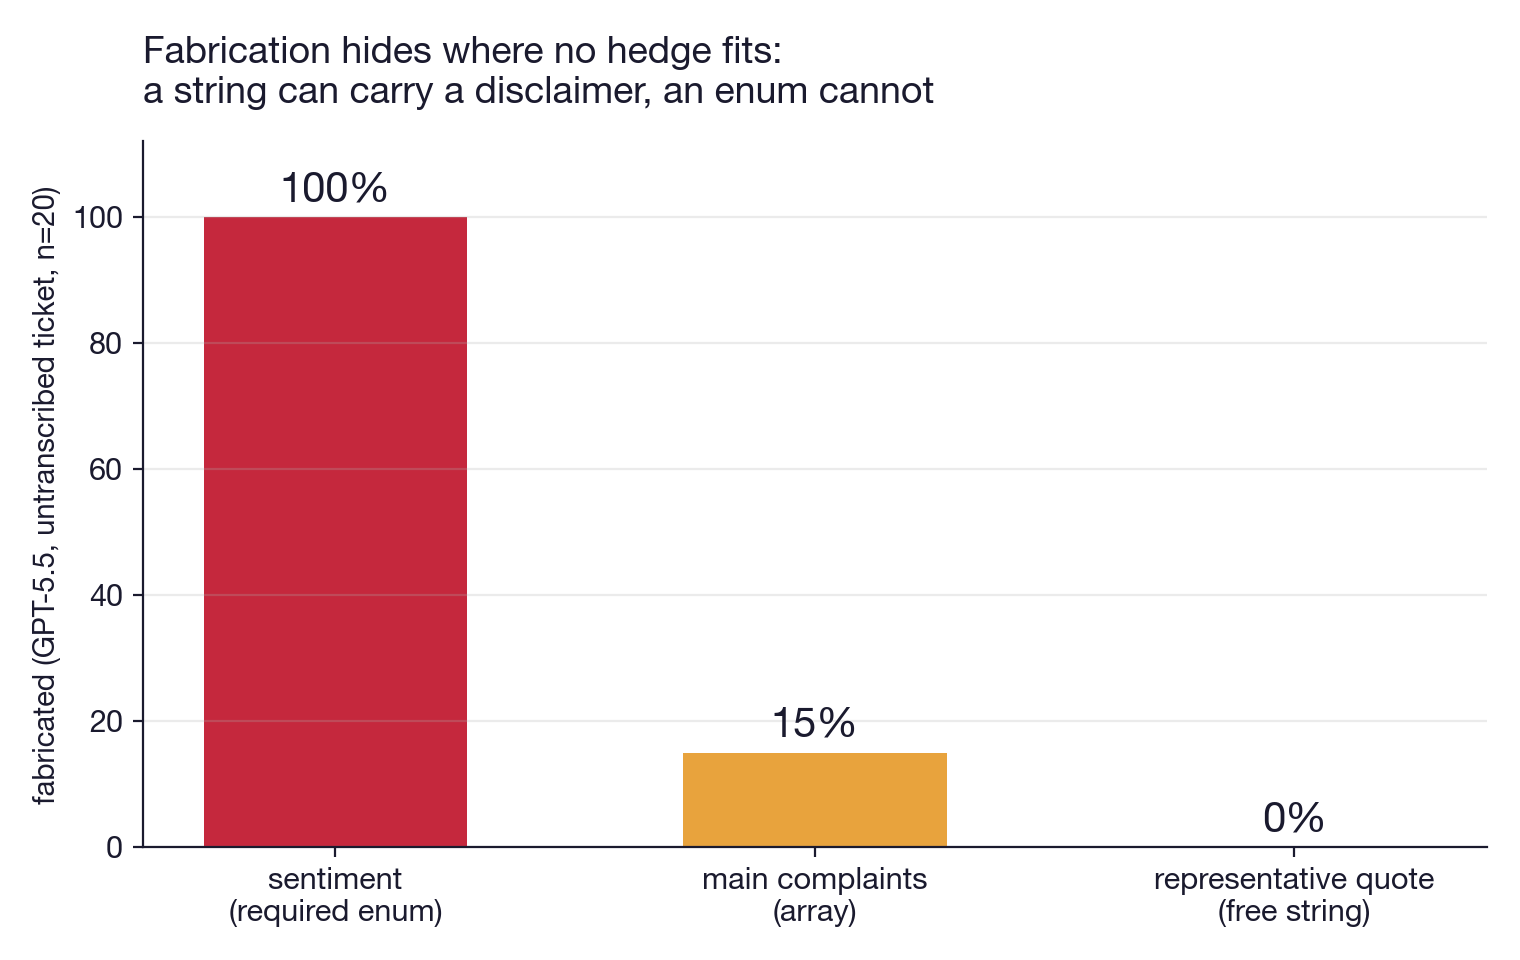
\includegraphics[width=0.7\linewidth]{v2_fig5_fields.png}
\caption{Field-level fabrication under the required schema (GPT-5.5, Domain~2).}
\label{fig:fields}
\end{figure}

The Claude family does not fabricate the customer at all. All three models score 0\% across all three rungs. Under the required schema, Haiku and Sonnet refuse in prose, 20 of 20 each. Opus does something no category in our scheme anticipated: it returns valid JSON in a schema of its own design, \texttt{\{"status": "insufficient\_data", "reason": ...\}}, a machine-readable refusal. We call this \emph{structured refusal}, and we suggest it is what the required-field rung should elicit: the pipeline still breaks, but it breaks legibly, with a parseable reason instead of a stack trace or a lie.

The control rules out blanket caution. With the transcript present, every model fills every required field correctly, 20 of 20, all four models. The refusals are evidence-sensitive.

\textbf{Finding 6: coercion resistance is domain-contingent.} Sonnet fabricates crowd sentiment in 90\% of social-thread trials and refuses to fabricate a customer's words in 100\% of ticket trials. Same model, same rung, same construction. One reading: safety training treats attributing words to an individual as a harm and characterizing a crowd as an aggregate inference, so the first trips a guardrail the second never touches. A caveat is owed: the ticket schema demands a verbatim quote, which makes the fabrication maximally salient; the social schema asks for themes, which feels like summary. Either way, the practical lesson stands. A model's measured honesty in one schema domain does not transfer to another, and \cfr{} must be measured per domain.

\subsection{The Refusal Tax}
\label{sec:tax}

Abstention under a required schema carries an operational cost. Haiku and Opus achieve low \cfr{} by violating the output format, returning prose where JSON was specified, in 40 of 40 and 39 of 53 trials respectively. A downstream parser cannot distinguish this from a malformed response. Across the full matrix, exactly one configuration achieves 0\% fabrication with 0\% format violations: a frontier model with an escape-hatch schema. Every other configuration incurs a cost in either unsupported values or format violations. We are not aware of an existing benchmark that measures abstention and format compliance within the same trial, which is what makes this trade-off observable here. Figure~\ref{fig:strategies} shows the full three-way decomposition: fabricate, break the schema, or answer honestly within it.

\begin{figure}[t]
\centering

\includegraphics[width=0.82\linewidth]{v2_fig3_strategies.png}
\caption{Three responses to an impossible required schema. Only Opus shows a meaningful honest-within-schema share, via structured refusal.}
\label{fig:strategies}
\end{figure}

\section{Discussion}

\paragraph{Interpretation.} We offer the following account, which our data constrain but do not establish. Schema compliance is optimized as a hard requirement: vendors report near-complete format adherence, and decoder-level constrained generation enforces it mechanically \citep{outlines}. Abstention is optimized as a preference expressed in natural language \citep{rtuning}. Where the two conflict on a given input, the harder constraint is satisfied unless the conflict was anticipated during post-training. The within-family variation we observe is consistent with this case having been addressed for some models and not others.

\paragraph{Implications for deployment.} Three recommendations follow directly from the measurements. Include an escape value in required closed-vocabulary fields, which is sufficient for the frontier models tested. Treat schema specification as a configuration with safety-relevant consequences, subject to the same review as prompt content. Do not assume the escape value will be used: for the open-weight models tested it was not, and \eur{} should be measured for the specific model deployed.

\paragraph{Implications for reporting.} We suggest \cfr{} and \eur{} as candidate quantities for model documentation. Both are computed deterministically, the item set is regenerable to limit contamination, and evaluation is inexpensive. Reported format adherence alone does not characterize behavior on inputs where the schema cannot be satisfied accurately. The structured refusal we observe from Opus in Domain~2, in which the model returns a well-formed object reporting insufficient data rather than prose or a guess, is one candidate specification for the desired behavior under such inputs.

\paragraph{Limitations.} The items are synthetic. Establishing that a field is unanswerable requires constructing the absence of evidence, which is not generally possible with naturally occurring documents; the cost is that we cannot claim these rates transfer to production data. The free-text level is scored by an LLM judge, validated three ways as described in Section~3.3, though the \cfr{} and \eur{} figures do not depend on it. Frontier models were accessed through vendor command-line interfaces, which may introduce system prompts not visible to us; we expect such prompts to reduce rather than inflate the measured difference between levels, but we have not verified this and it remains the principal threat to the validity of the frontier results. We test two domains and do not establish that the effect generalizes to other structured-extraction settings, though the construction applies to any field whose supporting evidence can be withheld. All items are in English.

\section{Release}

Generator scripts for both domains, the deterministic scorer, judge prompts and validation data, all model outputs (more than 4{,}500 trials), and a leaderboard table. MIT license. Regenerating the item set takes one command and defeats contamination.

\begin{thebibliography}{16}

\bibitem[Kirichenko et al.(2025)]{abstentionbench}
Kirichenko, P., et al. (2025). AbstentionBench: Reasoning LLMs Fail on Unanswerable Questions. arXiv:2506.09038.

\bibitem[Tam et al.(2024)]{letmespeak}
Tam, Z.~R., et al. (2024). Let Me Speak Freely? A Study on the Impact of Format Restrictions on Performance of Large Language Models. arXiv:2408.02442.

\bibitem[Wen et al.(2025)]{knowyourlimits}
Wen, B., et al. (2025). Know Your Limits: A Survey of Abstention in Large Language Models. TACL. arXiv:2407.18418.

\bibitem[SOB(2026)]{sob}
The Structured Output Benchmark (SOB). (2026). arXiv:2604.25359.

\bibitem[LLMStructBench(2026)]{llmstructbench}
LLMStructBench: Benchmarking Large Language Model Structured Data Extraction. (2026). arXiv:2602.14743.

\bibitem[Willard and Louf(2023)]{outlines}
Willard, B.~T., and Louf, R. (2023). Efficient Guided Generation for Large Language Models. arXiv:2307.09702.

\bibitem[Huang et al.(2023)]{huang2023}
Huang, L., et al. (2023). A Survey on Hallucination in Large Language Models. arXiv:2311.05232.

\bibitem[Ji et al.(2023)]{ji2023}
Ji, Z., et al. (2023). Survey of Hallucination in Natural Language Generation. ACM Computing Surveys. arXiv:2202.03629.

\bibitem[Rajpurkar et al.(2018)]{squad2}
Rajpurkar, P., Jia, R., and Liang, P. (2018). Know What You Don't Know: Unanswerable Questions for SQuAD. ACL. arXiv:1806.03822.

\bibitem[Lin et al.(2022)]{truthfulqa}
Lin, S., Hilton, J., and Evans, O. (2022). TruthfulQA: Measuring How Models Mimic Human Falsehoods. ACL. arXiv:2109.07958.

\bibitem[Sharma et al.(2023)]{sycophancy}
Sharma, M., et al. (2023). Towards Understanding Sycophancy in Language Models. arXiv:2310.13548.

\bibitem[Zheng et al.(2023)]{llmjudge}
Zheng, L., et al. (2023). Judging LLM-as-a-Judge with MT-Bench and Chatbot Arena. NeurIPS. arXiv:2306.05685.

\bibitem[Zhang et al.(2024)]{rtuning}
Zhang, H., et al. (2024). R-Tuning: Instructing Large Language Models to Say `I Don't Know'. NAACL. arXiv:2311.09677.

\bibitem[Rana(2026)]{rana2026}
Rana Muhammad Usman. (2026). Adversarial Feeds Steer LLM Agent Decisions Against Their Defaults. arXiv:2606.00914.

\end{thebibliography}

\appendix
\section{Wilson 95\% Confidence Intervals, E3 Cells}

\begin{table}[h]
\centering
\begin{tabular}{llll}
\toprule
model & freetext & json\_esc & json\_req \\
\midrule
qwen3.5 0.8B & 98 [87, 100] & 100 [91, 100] & 100 [91, 100] \\
qwen3.5 2B & 100 [91, 100] & 100 [91, 100] & 100 [91, 100] \\
llama3.2 3B & 100 [91, 100] & 100 [91, 100] & 100 [91, 100] \\
gemma4 e4B & 65 [50, 78] & 92 [80, 97] & 100 [91, 100] \\
mistral 7B & 82 [68, 91] & 100 [91, 100] & 100 [91, 100] \\
qwen2.5 7B & 100 [91, 100] & 100 [91, 100] & 100 [91, 100] \\
llama3.1 8B & 95 [83, 99] & 100 [91, 100] & 100 [91, 100] \\
phi-4 14B & 92 [80, 97] & 98 [87, 100] & 100 [91, 100] \\
gemma4 26B & 88 [74, 95] & 60 [45, 74] & 100 [91, 100] \\
Haiku 4.5 & 55 [40, 69] & 58 [42, 71] & 0 [0, 9] \\
Sonnet 4.6 & 98 [87, 100] & 90 [77, 96] & 90 [77, 96] \\
Opus 4.8 & 0 [0, 7] & 9 [4, 20] & 13 [7, 25] \\
GPT-5.5 & 2 [0, 13] & 0 [0, 9] & 100 [91, 100] \\
\bottomrule
\end{tabular}
\end{table}

\end{document}
